\documentclass[tikz,border=2pt]{standalone}
\pdfmapfile{+cm.map}
\usepackage{pgfplots}
\pgfplotsset{compat=1.18}
\usetikzlibrary{arrows.meta}
\definecolor{ink}{HTML}{202B30}
\definecolor{red}{HTML}{971D2C}
\definecolor{soft}{HTML}{F4E9EB}
\definecolor{gray}{HTML}{51636D}
\definecolor{line}{HTML}{D6DDE0}
\definecolor{pale}{HTML}{F0F3F4}
\begin{document}
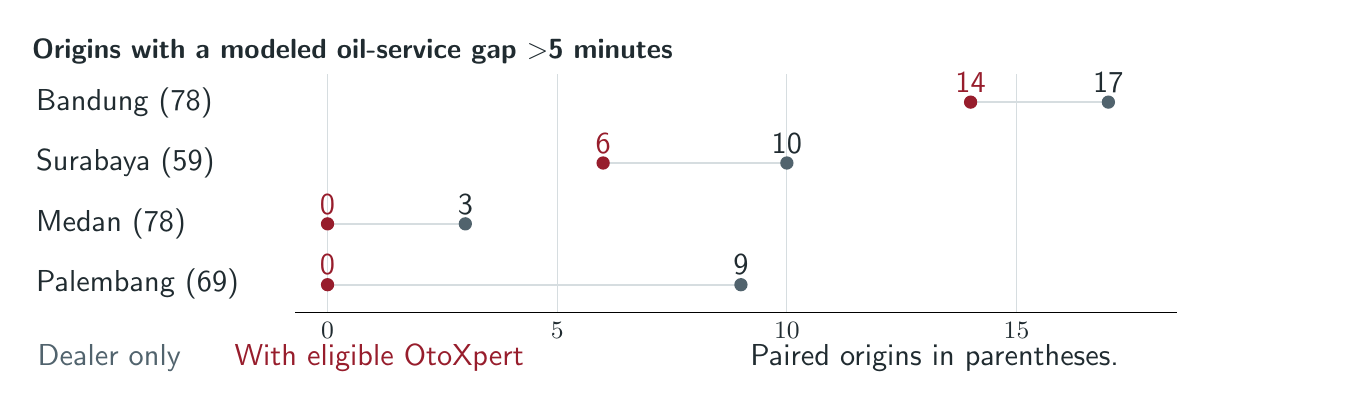
\begin{tikzpicture}[x=1cm,y=1cm,font=\sffamily\fontsize{10.5}{12}\selectfont,text=ink,arr/.style={-{Stealth[length=2mm]},draw=gray,thick}]
\path[use as bounding box] (0,0) rectangle (16.4,4.42);
\node[anchor=west,inner sep=0pt,font=\sffamily\bfseries] at (0.05,4.12) {Origins with a modeled oil-service gap $>$5 minutes};
\begin{axis}[at={(3.4cm,.8cm)},anchor=south west,width=11.2cm,height=3.03cm,scale only axis,xmin=-.7,xmax=18.5,ymin=.54,ymax=4.46,ytick={1,2,3,4},yticklabels={Palembang (69),Medan (78),Surabaya (59),Bandung (78)},xtick={0,5,10,15},tick style={draw=none},axis x line*=bottom,axis y line=none,xmajorgrids,grid style={line},tick label style={font=\sffamily\small},clip=false]\draw[thick,line] (axis cs:0,1) -- (axis cs:9,1);\fill[red] (axis cs:0,1) circle (2.4pt);\fill[gray] (axis cs:9,1) circle (2.4pt);\node[above,text=red] at (axis cs:0,1) {0};\node[above] at (axis cs:9,1) {9};\draw[thick,line] (axis cs:0,2) -- (axis cs:3,2);\fill[red] (axis cs:0,2) circle (2.4pt);\fill[gray] (axis cs:3,2) circle (2.4pt);\node[above,text=red] at (axis cs:0,2) {0};\node[above] at (axis cs:3,2) {3};\draw[thick,line] (axis cs:6,3) -- (axis cs:10,3);\fill[red] (axis cs:6,3) circle (2.4pt);\fill[gray] (axis cs:10,3) circle (2.4pt);\node[above,text=red] at (axis cs:6,3) {6};\node[above] at (axis cs:10,3) {10};\draw[thick,line] (axis cs:14,4) -- (axis cs:17,4);\fill[red] (axis cs:14,4) circle (2.4pt);\fill[gray] (axis cs:17,4) circle (2.4pt);\node[above,text=red] at (axis cs:14,4) {14};\node[above] at (axis cs:17,4) {17};\end{axis}\node[anchor=west,inner sep=0pt,text=gray] at (0.12,0.22) {Dealer only};
\node[anchor=west,inner sep=0pt,text=red] at (2.62,0.22) {With eligible OtoXpert};
\node[anchor=west,inner sep=0pt,] at (9.17,0.22) {Paired origins in parentheses.};
\node[anchor=west,inner sep=0pt,] at (0.1,3.47) {Bandung (78)};
\node[anchor=west,inner sep=0pt,] at (0.1,2.7) {Surabaya (59)};
\node[anchor=west,inner sep=0pt,] at (0.1,1.93) {Medan (78)};
\node[anchor=west,inner sep=0pt,] at (0.1,1.16) {Palembang (69)};
\end{tikzpicture}\end{document}